\chapter{Data and Pre-Processing}%
\label{sec:data}

Geographic data is in wide use by both the public and private sector, and is a huge subject in and of itself.
The storage, processing, and inspection of such data is handled by \textit{Geographic Information Systems} (GIS).
In this section we will explain a few core GIS concepts relevant for the problem at hand, concepts which will inform decisions for how to prepare the data for machine learning purposes.
\Cref{sec:coordinate-systems} will give a brief introduction to the coordinate systems used to represent geographic data.
GIS data can be largely bisected into two categories, vector data and raster data, and both types will be described in \cref{sec:data-types}.
\Cref{sec:data-sets} will present the datasets used for training our models.
The remaining subsections will describe the preprocessing pipeline which has been developed for our specific purposes, preprocessing in the form of cadastral tiling (\cref{sec:tiling-algorithm}), segmentation masking (\cref{sec:masking-algorithm}), and surface rasterization (\cref{sec:surface-rasterization}).
A figurative overview of the preprocessing pipeline is provided by \cref{fig:preprocessing-overview} in \cref{app:preprocessing-overview}.


\section{Coordinate Systems}%
\label{sec:coordinate-systems}
One of the most common coordinate system for representing \textit{arbitrary} positions on earth's surface is the \textit{geographic coordinate system} (GPS).
A given point, $\vec{p} = (\phi, \lambda, z)$, is represented by an angular latitude and longitude, $\phi$ and $\lambda$ respectively, and a radial distance from the mean sea level, $z$.
A negative value for $z$ does not necessarily imply that the given point is below ground, as certain areas (such as in the Netherlands) are situated below sea level.
It is therefore not sufficient to represent elevation data with unsigned floating point numbers.

Although GPS is able to uniquely represent arbitrary geographic points with a high degree of accuracy, it is still unsuitable for many applications.
Cartesian transformations and distance norms are cumbersome to calculate, and data structures and visualizations which are fundamentally two dimensional in nature, such as maps, rasters, and matrices, are difficult to construct from spherical coordinates while protecting important properties of the data.

\begin{wrapfigure}[17]{r}{0.38\linewidth}
  \centering
  \includegraphics[width=0.9\linewidth]{europe-utm-zones.png}
  \caption[UTM zones covering Europe.]{%
    The figure shows the UTM zones required in order to cover the entirety of Europe, from \texttt{29S} to \texttt{38W}.
    This public domain image has been sourced from Wikimedia~\cite{wiki:europe_utm_zones}.
  }%
  \label{fig:europe-utm-zones}
\end{wrapfigure}

In order to solve this problem we define a set of coordinate system \textit{projections} which approximate predefined regions of the earth's surface as flat planes.
The resulting coordinate systems are Cartesian and thus allow us to represent geographic points in the more common $\vec{p} = (x, y, z)$ format.
Cartesian distance norms such as $||\vec{p}_1 - \vec{p}_2||_2$ and Cartesian translations $\vec{p}_1 + \vec{p}_2$ stay within predefined error tolerances as long as operations are contained to the validity region of the given projection.

One such Cartesian approximation of the earth's surface is the Universal Transverse Mercator (UTM) coordinate system which divides the earth into 60 rectangular zones~\cite[p.~48]{map-projections}. The UTM zones covering Europe are shown in \cref{fig:europe-utm-zones}.
We will exclusively use UTM zone \texttt{32V} for our datasets covering the municipality of Trondheim situated in the southern part of Norway.
Data provided in alternative coordinate systems will be mapped to this UTM zone before we start using the data.
Since this is an affine coordinate system, we can easily generalize any models to other coordinate systems by applying the correct affine transformations.
Technical details for how to map between different coordinate systems are given in \cref{app:srid-change} for reproducibility.


\section{Data Types}%
\label{sec:data-types}

We will provide a brief overview of the two main categories of GIS data, namely \textit{vector data} and \textit{raster data}, and how to prepare these data types for machine learning purposes.

\subsection{Vector data}%
\label{sec:vector-data}
A \textit{line string} is an ordered collection of geographic points $(\vec{p}_0, \ldots, \vec{p}_n)$ defining a path which connects each consecutive point by a straight line.
The points are therefore necessarily order dependent.
A \textit{simple} line string is a path which does \textit{not} intersect itself, while a \textit{complex} line string is one that does.
When the first and last points of a line string are identical it is considered a \textit{linear ring}, i.e.\ $l = (\vec{p}_0, \ldots, \vec{p}_n, \vec{p}_0)$.
A \textit{polygon} can therefore be represented by a simple linear ring which defines its \textit{exterior hull} and any number of simple linear strings which defines its \textit{interior hulls}.
\Cref{fig:polygon-representation} illustrates these concepts for polygons with and without interior hulls. % chktex 2

\begin{figure}[H]
  \centering
  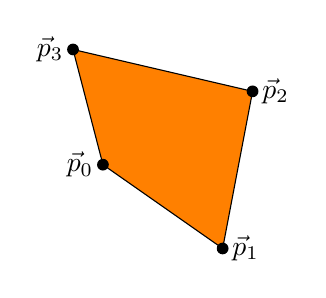
\begin{tikzpicture}[scale=1.9,yscale=0.7]
  \coordinate (zero) at (0, 0);
  \coordinate (one) at (0.8, -0.8);
  \coordinate (two) at (1, 0.7);
  \coordinate (three) at (-0.2, 1.1);
  \draw[fill=orange]
    (zero) node[left] {$\vec{p}_0$}
    -- (one) node[right] {$\vec{p}_1$}
    -- (two) node[right] {$\vec{p}_2$}
    -- (three) node[left] {$\vec{p}_3$}
    -- cycle;
  \foreach \n in {zero,one,two,three}
    \node at (\n)[circle,fill,inner sep=1.5pt]{};
\end{tikzpicture}

  \textcolor{gray}{\vrule}
  \hspace{0.01\linewidth}
  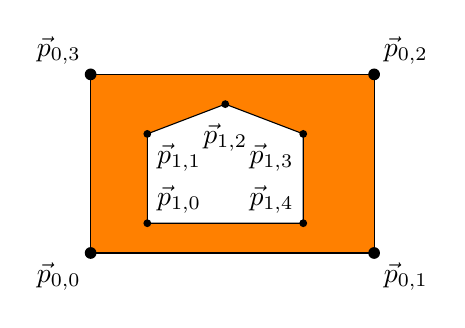
\begin{tikzpicture}[scale=1.8,yscale=0.7]
  \coordinate (zero) at (0, 0);
  \coordinate (one) at (2.0, 0);
  \coordinate (two) at (2.0, 1.8);
  \coordinate (three) at (0, 1.8);
  \draw[fill=orange]
    (zero) node[below left] {$\vec{p}_{0,0}$}
    -- (one) node[below right] {$\vec{p}_{0,1}$}
    -- (two) node[above right] {$\vec{p}_{0,2}$}
    -- (three) node[above left] {$\vec{p}_{0,3}$}
    -- cycle;
  \foreach \n in {zero,one,two,three}
    \node at (\n)[circle,fill,inner sep=1.5pt]{};

  \coordinate (0) at (0.4, 0.3);
  \coordinate (1) at (1.5, 0.3);
  \coordinate (2) at (1.5, 1.2);
  \coordinate (3) at (0.95, 1.5);
  \coordinate (4) at (0.4, 1.2);
  \draw[fill=white]
    (0) node[above right] {$\vec{p}_{1,0}$}
    -- (1) node[above left] {$\vec{p}_{1,4}$}
    -- (2) node[below left] {$\vec{p}_{1,3}$}
    -- (3) node[below=3.5pt] {$\vec{p}_{1,2}$}
    -- (4) node[below right] {$\vec{p}_{1,1}$}
    -- cycle;
  \foreach \n in {0,1,2,3,4}
    \node at (\n)[circle,fill,inner sep=1pt]{};
\end{tikzpicture}

  \caption[Types of vectorized polygons.]{%
    Simple polygon with four unique vertices is shown on the left hand side.
    A complex polygon with an outer hull
    and an interior hull is shown on the right hand side for comparison.
  }%
  \label{fig:polygon-representation}
\end{figure}

A polygon is considered invalid if one or more of its linear rings are self-intersecting, i.e.\ if any of its rings is considered to be complex.
Data providers frequently provide polygons in invalid states and such polygons must be corrected since they are often not processable by common GIS tools.
Zero-buffering invalid polygons (growing the polygon in all directions by zero units) fixes such problems, as can be seen in \cref{fig:complex-zero-buffer}.

\begin{figure}[H]
  \centering
  \begin{tikzpicture}[scale=1]
  \coordinate (ll) at (0, 0);
  \coordinate (mid) at (2, 1);
  \coordinate (lr) at (4, 0);
  \coordinate (ur) at (4, 2);
  \coordinate (ul) at (0, 2);
  \draw[fill=orange]
    (ll) node[left] {$\vec{p}_0$}
    -- (ur) node[right] {$\vec{p}_1$}
    -- (lr) node[right] {$\vec{p}_2$}
    -- (ul) node[left] {$\vec{p}_3$}
    -- cycle;
  \foreach \n in {ll,ur,lr,ul}
    \node at (\n)[circle,fill,inner sep=1.5pt]{};

   \draw (4.4, 1) edge[->, thick] node[above] {\texttt{buffer(0.0)}} (6.6, 1);

  \coordinate (offset) at (7, 0);
  \draw[fill=orange]
    ($ (ll) + (offset) $) node[left] {$\vec{p}_0$}
    -- ($ (mid) + (offset) $) node[below] {$\vec{p}_1$}
    -- ($ (lr) + (offset) $) node[right] {$\vec{p}_2$}
    -- ($ (ur) + (offset) $) node[right] {$\vec{p}_3$}
    -- ($ (mid) + (offset) $) node[above] {$\vec{p}_4$}
    -- ($ (ul) + (offset) $) node[left] {$\vec{p}_5$}
    -- cycle;
  \foreach \n in {ll,mid,lr,ur,mid,ul}
    \node at ($ (\n) + (offset) $)[circle,fill,inner sep=1.5pt]{};
\end{tikzpicture}

  \caption{Illustration of how zero-buffering an invalid polygon corrects self-intersecting polygons.}%
  \label{fig:complex-zero-buffer}
\end{figure}

Zero-buffering polygons has the added benefit of normalizing vector data by re-ordering the polygon vertices in an anti-clockwise manner and removing redundant vertices as shown in \cref{fig:redundant-zero-buffer}.

\begin{figure}[H]
  \centering
  \begin{tikzpicture}[scale=1]
  \coordinate (ll) at (0, 0);
  \coordinate (lm) at (2, 0);
  \coordinate (lr) at (4, 0);
  \coordinate (ur) at (4, 1);
  \coordinate (um) at (2, 1);
  \coordinate (Um) at (2, 2);
  \coordinate (ul) at (0, 1);
  \draw[fill=orange]
    (ll) node[below] {$\vec{p}_0$}
    -- (lm) node[below] {$\vec{p}_1$}
    -- (lr) node[below] {$\vec{p}_2$}
    -- (ur) node[above] {$\vec{p}_3$}
    -- (um) node[above right] {$\vec{p}_4$}
    -- (Um) node[above] {$\vec{p}_5$}
    -- (um) node[above left] {$\vec{p}_6$}
    -- (ul) node[above] {$\vec{p}_7$}
    -- cycle;
  \foreach \n in {ll,lm,lr,ur,um,Um,um,ul}
    \node at (\n)[circle,fill,inner sep=1.5pt]{};

   \draw (4.9, 0.5) edge[->, thick] node[above] {\texttt{buffer(0.0)}} (7.1, 0.5);

  \coordinate (offset) at (8, 0);
  \draw[fill=orange]
    ($ (ll) + (offset) $) node[below] {$\vec{p}_0$}
    -- ($ (lr) + (offset) $) node[below] {$\vec{p}_1$}
    -- ($ (ur) + (offset) $) node[above] {$\vec{p}_2$}
    -- ($ (ul) + (offset) $) node[above] {$\vec{p}_3$}
    -- cycle;
  \foreach \n in {ll,lr,ur,ul}
    \node at ($ (\n) + (offset) $)[circle,fill,inner sep=1.5pt]{};
\end{tikzpicture}

  \caption{Illustration of how zero-buffering polygons removes redundant vertices.}%
  \label{fig:redundant-zero-buffer}.
\end{figure}

This allows you to apply simpler similarity measures for comparing polygons, and reduces computational costs when processing the polygons.
Technical details for applying zero-buffers to vector data is provided in \cref{app:zero-buffer}.
We will come back to how to combine vector and raster datasets by \textit{rasterization} in \cref{sec:masking-algorithm} where it will also become clear why the removal of redundant vertices is of importance.


\subsection{Raster data}%
\label{sec:raster-data}
Raster data consists of a set of scalar measurements imposed onto a grid.
A color image, $\rgbraster$, of width $\mathrm{W}$ and height $\mathrm{H}$, will contain three color channels; red, green, and blue (RGB), and can be represented by a three-dimensional array of size $\mathrm{H} \times \mathrm{W} \times \mathrm{3}$.
Each color channel for a given pixel is represented by an unsigned 8-bit integer, i.e.
%
\begin{equation*}
  \rgbraster_{i, j, c} \in \{0, 1, \ldots, 255\},
  \hspace{2.5em}
  i = 1, \ldots, \mathrm{H} ,
  ~~
  j = 1, \ldots, \mathrm{W},
  ~~
  c = \mathrm{\textcolor{red}{r}, \textcolor{green}{g}, \textcolor{blue}{b}}.
\end{equation*}
%
A LiDAR elevation map, which we will denote as $\lidarraster$, is likewise encoded as a single-channel grayscale image of size $\mathrm{W} \times \mathrm{H}$.
Each pixel is represented by a signed 32-bit floating point value which gives the following approximate value domain
%
\begin{equation*}
  \lidarraster_{i, j} \in \mathbb{R},
  \hspace{2.5em}
  i = 0, \ldots, \mathrm{H} - 1,
  ~~
  j = 0, \ldots, \mathrm{W} - 1.
\end{equation*}
%
These two raster types must be handled differently during data-standardization and -normalization due to their different value domains, which we will come back to in \cref{sec:raster-normalization}.
Whenever we refer to remote sensing raster data in \emph{general}, be it LiDAR and/or RGB, we will denote the input raster as $\inputraster$.

For GIS rasters specifically we must additionally provide the spatial extent of the given raster defined by:
\begin{itemize}[noitemsep]
  \item A coordinate system, for example UTM \texttt{32V}.
  \item The coordinate of the center of the upper left pixel, $\inputraster_{1, 1}$; the \textit{origin} $\vec{r}_0 = {[x_0, y_0]}^T$.
  \item The pixel step size, $\vec{\Delta} = {[\Delta_x, \Delta_y]}^T$, for example ${[\SI{0.25}{\meter}, \SI{-0.25}{\meter}]}^T$.
\end{itemize}

The pixel value $\inputraster_{i, j, c}$ therefore represents a rectangle of width $\Delta_x$ and height $\Delta_y$ centered at the spatial coordinate $\vec{r}_0 + [\Delta_y i, \Delta_x j]$ interpreted in the given coordinate system.

Missing data in remote sensing rasters is specified by filling in a predefined \texttt{nodata} placeholder value.
For RGB data this is often set to $0$, resulting in a black pixel.
LiDAR rasters often use $\texttt{nodata} = -2^{127} \times (2 - 2^{-23}) \approx -3.4028234664 \times 10^{38}$, the most negative normal number representable by a single-precision floating point number.
Such \texttt{nodata} values may arise from measurement errors or by pixels situated outside the given coverage area of the dataset, and must be special-cased during data normalization, which we will come back to in \cref{sec:raster-normalization}.

When we will train models on the combination of LiDAR and aerial photography data, these two types of rasters must be merged in order to attain a consistent three-dimensional array of size $H \times W \times 4$.
These rasters can not be simply superposed when their pixel sizes $\vec{\Delta}$ and/or origins $\vec{r}_0$ differ.
In such cases we will apply bilinear interpolation on the raster of greatest resolution and subsequently downsample it in order to align all pixels.
See \cref{app:raster-merging} for how this is performed in practice.


\section{Datasets}%
\label{sec:data-sets}

The modelling results presented in \cref{sec:experiments} are trained on GIS data covering the Norwegian municipality of Trondheim.
All datasets have been made available by the \enquote{Norge digitalt}-partnership and have been downloaded from \url{https://geonorge.no}, an online service hosted by \textit{Norwegian Mapping and Cadastre Authority} (\textit{Statens Kartverk}).
All data, unless otherwise stated, are licenced under the \enquote{Norge digitalt}-licence\footnote{Information regarding the \enquote{Norge digitalt}-licence can be found here: \url{https://www.geonorge.no/Geodataarbeid/Norge-digitalt/Avtaler-og-maler/Norge-digitalt-lisens/}.} which restricts the use to non-commercial purposes.

\subsection{Raster datasets}
We will use the \enquote{Ortofoto Trondheim 2017}\footnote{Product specification for \enquote{Ortofoto Trondheim 2017} can be found here:\\ \url{https://kartkatalog.geonorge.no/metadata/cd105955-6507-416f-86d2-6d95c1b74278}.} aerial photography dataset from 2017 which requires \SI{161}{\giga\byte} of storage space.
The real image resolution is \SIrange{0.04}{0.15}{\meter}, but is provided with an resampled resolution of \SI{0.1}{\meter} for consistency, that is, each pixel is of size $\SI{0.1}{\meter} \times \SI{0.1}{\meter}$.
The reported accuracy is \SI{\pm 0.35}{\meter}~\cite{trondheim_ortophoto_2017}, although the exact type of this accuracy is not specified.
An exemplified region is visualized in \cref{fig:rgb-example}.

\begin{figure}[hbt]
  \centering
  \includegraphics[width=0.75\linewidth]{data/rgb-example}
  \appcaption{%
    Visualization of the \enquote{Ortofoto Trondheim 2017} aerial photography dataset.
  }{%
    \copyright{Kartverket}.
  }%
  \label{fig:rgb-example}
\end{figure}

An \textit{orthophoto} is an image where the geographic scale is uniform over the entire image.
Proper orthophotos are expensive to manufacture and are therefore seldomly available for most geographic regions~\cite{ortofoto_in_norway_2003}, including Trondheim.
Aerial photography which has not been properly \enquote{ortho-rectified} may impede location-based inference as there exists no exact one-to-one mapping between image pixels and geographic coordinates.
This problem is best understood by an example, as shown in \cref{fig:non-orthophoto-example}.

\begin{figure}[hbt]
  \centering
  \begin{tikzpicture}
    \node[anchor=south west,inner sep=0] (image) at (0,0) {\includegraphics[width=0.75\linewidth]{data/non-orthophoto-example}};
    \begin{scope}[x={(image.south east)},y={(image.north west)}]
      \draw[orange, ultra thick, fill=orange!50, fill opacity=0.25]
        (0.34, 0.3) --
        (0.615, 0.55) --
        (0.61, 0.69) --
        (0.33, 0.445) --
        cycle;
    \end{scope}
  \end{tikzpicture}
  \appcaption{%
    Example of nonproper orthophoto.
  }{%
    The building centered in the image is 14 stories tall.
    The orange area annotates a clearly visible building wall.
    \copyright{Kartverket}.
  }%
  \label{fig:non-orthophoto-example}
\end{figure}

As can be seen in \cref{fig:non-orthophoto-example}, the \enquote{Ortofoto Trondheim 2017} dataset clearly shows one side of a building due to the perspective of the plane capturing the image.
An ideal orthophoto would capture all vertical building walls as single, straight lines, no matter the perspective.
The effect of this \enquote{parallax error} on semantic segmentation predictions has been investigated in our previous work~\cite{specialization-project}, the conclusion being that it does \emph{not} impede predictive accuracy to a major degree.

The LiDAR dataset used is \enquote{Høydedata Trondheim 5pkt 2017}\footnote{Product specification for \enquote{Høydedata Trondheim 5pkt 2017} can be found here:\\ \url{https://kartkatalog.geonorge.no/metadata/bec4616f-9a62-4ecc-95b0-c0a4c29401dc}.} from \date{2017-10-10} and requires \SI{25}{\giga\byte} of storage space.
The pixel size is $\SI{0.25}{\meter} \times \SI{0.25}{\meter}$ and the LiDAR measurements have a reported standard deviation of \SI{0.02}{\meter}~\cite{trondheim_lidar_2017}.
LiDAR visualized as a grayscale image over the same region as in \cref{fig:rgb-example} is presented in \cref{fig:lidar-example}.

\begin{figure}[hbt]
  \centering
  \includegraphics[width=0.75\linewidth]{data/lidar-example}
  \caption[Visualization of LiDAR data from Trondheim.]{%
    Visualization of the \enquote{Høydedata Trondheim 5pkt 2017} LiDAR dataset.
    \copyright{Kartverket}.
  }%
  \label{fig:lidar-example}
\end{figure}


\subsection{Vector datasets}
The \enquote{Matrikkelen - Eiendomskart Teig}\footnote{Product specification for \enquote{Matrikkelen - Eiendomskart Teig} can be found here:\\\url{https://kartkatalog.geonorge.no/metadata/74340c24-1c8a-4454-b813-bfe498e80f16}.} data set contains all cadastral plots in Trondheim, the use of which will be explained in \cref{sec:tiling-algorithm}.
The \enquote{FKB-bygning}\footnote{Product specification for \enquote{FKB-bygning} can be found here:\\\url{https://kartkatalog.geonorge.no/metadata/8b4304ea-4fb0-479c-a24d-fa225e2c6e97}.} data set contains all registered building outlines in Trondheim.
The building outlines will be used to construct binary classification masks as outlined in \cref{sec:masking-algorithm}.
Both data sets are illustrated in \cref{fig:vector-data-example}.

\begin{figure}[htb]
  \includegraphics[trim={5cm 0 5cm 0},clip, width=0.49\linewidth]{data/teig-example}
  \includegraphics[trim={5cm 0 5cm 0},clip, width=0.49\linewidth]{data/building-example}
  \caption{%
    Illustration of vector data sets.
    Cadastral plots are shown on the left while building outlines are shown on the right.
    \copyright{Kartverket}.
  }%
  \label{fig:vector-data-example}
\end{figure}


\section{Tiling Algorithm}%
\label{sec:tiling-algorithm}
The data sets provided to us are in a state unsuitable for direct use by machine learning frameworks.
For this reason we need to develop a preprocessing pipeline that transforms the data into a more customary format.
The data preprocessing should be generalizable to different regions, data formats, data types (vector vs.\ raster), coordinate systems, and so on.
The goal is to implement a modelling pipeline that can be applied to other geographic regions in the future.

Our data sets are defined over a single, contiguous geographic area, and we must therefore define a \textit{sample space} which allows us to split the data into training-, validation-, and test-sets.
The collection of all cadastral plots in a given region is a suitable sample space since cadastral plots are non-overlapping regions of relatively small size and have a high probability of containing one or more buildings.
A large raster dataset covering a sparsely populated region can therefore be substantially reduced in size before training.
An alternative approach is to split the entire data set into regularly sized tiles and use this tile collection as the sample space.
A tiled sample space, for anything other than densely populated areas, will suffer from class imbalances due to low building densities in most tiles.

Given a specific geographic region, defined by the extent of the cadastral plot, we must retrieve the raster which covers the region of interest.
The simplest approach is to calculate the \textit{axis-aligned bounding box} of the plot, the minimum-area enclosing rectangle of the given plot.
A bounding box is uniquely defined by its centroid $\vec{c} = [\nicefrac{1}{2}(x_{\mathrm{\min}} + x_{\mathrm{\max}}), \nicefrac{1}{2}(y_{\mathrm{\min}} + y_{\mathrm{\max}})]$, width $w = x_{\mathrm{\max}} - x_{\mathrm{\min}}$, and height $h = y_{\mathrm{\max}} - y_{\mathrm{\min}}$, and we will denote it by $B(\vec{c}, w, h)$.
This is shown in \cref{fig:cadastral-bbox}.

\begin{figure}[htb]
  \captionsetup[subfigure]{position=b}
  \centering
  \subcaptionbox{
    Bounding box calculation for a given cadastral.
    The cadastral is shown in \textcolor{orange}{orange},
    and the resulting bounding box is annotated with \textcolor{blue}{blue} dashed lines.%
    \label{fig:cadastral-bbox}
  }{
    \begin{tikzpicture}[scale=0.035]
  \tikzmath{
    \xmin=0;
    \xmax=100;
    \ymin=0;
    \ymax=100;
    \xmid=0.5 * \xmin + 0.5 * \xmax;
    \ymid=0.5 * \ymin + 0.5 * \ymax;
  }
  \coordinate (lr) at (\xmax, \ymin);
  \coordinate (ul) at (\xmin, \ymax);

  \draw[dashed, color=cadastralcolor, fill=cadastralcolor!10] (\xmin, \ymin) rectangle (\xmax, \ymax);
  \filldraw[orange, draw=black] (50, \ymin) -- (62.5, 12.5) -- (25, 50) -- (\xmax, 50) -- (50, \ymax) -- (0, 50) -- cycle;

  \draw (ul) node[above] {$(x_{\mathrm{min}}, y_{\mathrm{max}})$};
  \fill[cadastralcolor] (ul) circle [radius=1];

  \draw (lr) node[below] {$(x_{\mathrm{max}}, y_{\mathrm{min}})$};
  \fill[cadastralcolor] (lr) circle [radius=1];

  \draw (\xmid, \ymax) node[above] {$\hspace{3em}w = x_{\mathrm{max}} - x_{\mathrm{min}}$};
  \draw (\xmax, \ymid) node[above, rotate=-90] {$\hspace{-3em}h = y_{\mathrm{max}} - y_{\mathrm{min}}$};

  \draw (\xmid, 65) node[scale=1, black] {\textsf{CADASTRAL}};
\end{tikzpicture}

  }
  \hspace{2em}
  \subcaptionbox{
    Figure showing the difference between a regular bounding box shown in
    \textcolor{blue}{blue}, and a minimum rotated rectangle shown in
    \textcolor{red}{red}.
    Angle of rectangle rotation denoted by $\phi$.%
    \label{fig:rotated-bbox}
  }{
    \begin{tikzpicture}[scale=0.035]
  \tikzmath{
    \xmin=0;
    \xmax=100;
    \ymin=0;
    \ymax=100;
    \xmid=0.5 * \xmin + 0.5 * \xmax;
    \ymid=0.5 * \ymin + 0.5 * \ymax;
  }
  \coordinate (lr) at (\xmax, \ymin);
  \coordinate (ul) at (\xmin, \ymax);

  \draw[dashed, color=cadastralcolor, fill=cadastralcolor!10] (\xmin, \ymin) rectangle (\xmax, \ymax);
  \draw[dashed, color=red, fill=red!20, fill opacity=1] (\xmin, 50) -- (50, \ymin) -- (\xmax, 50) -- (50, \ymax) -- cycle; 
  \filldraw[orange, draw=black] (50, \ymin) -- (62.5, 12.5) -- (25, 50) -- (\xmax, 50) -- (50, \ymax) -- (0, 50) -- cycle;
  \draw[dashed, thick, color=red] (\xmin, 50) -- (50, \ymin) -- (\xmax, 50) -- (50, \ymax) -- cycle; 

  \fill[cadastralcolor] (ul) circle [radius=1];
  \fill[cadastralcolor] (lr) circle [radius=1];

  \fill[red] (\xmin, 50) circle [radius=1];
  \fill[red] (\xmax, 50) circle [radius=1];

  % Draw angle of rotation
  \draw[black] (\xmid + 20, \ymax) arc [start angle=0, end angle=-45, radius=20] node[midway, right] {$\phi$};

  % The following is added such that the resulting figure has the same dimensions as cadastre_bbox
  \draw (ul) node[above] {$(x_{\mathrm{min}}, y_{\mathrm{max}})$};
  \fill[cadastralcolor] (ul) circle [radius=1];
  \draw (lr) node[below] {$(x_{\mathrm{max}}, y_{\mathrm{min}})$};
  \fill[cadastralcolor] (lr) circle [radius=1];
\end{tikzpicture}

  }
  \caption{Comparison of bounding box methods.}
\end{figure}

The edges of the bounding box is by definition oriented parallel to the coordinate axes.
An alternative method is to calculate the \textit{arbitrarily oriented minimum bounding box} (AOMBB), a rectangle rotated by $\phi$ degrees w.r.t.\ the $x$-axis, as shown in \cref{fig:rotated-bbox}.

While AOMBB yields regions with less superfluous raster data, it requires warping of the original raw raster whenever $\phi$ is not a multiple of \SI{90}{\degree}, i.e.\ $\phi \not\in \{ \SI{0}{\degree}, \SI{90}{\degree}, \SI{180}{\degree}, \SI{270}{\degree} \}$.
Such warping requires data interpolation of the original raster data due to the rotation of the coordinate system, and may introduce artifacts to the warped raster without careful parameter tuning.
AOMBB is therefore not a viable approach during the preprocessing stage, and we will therefore use axis-aligned minimum bounding boxes instead, from now on simply referred to as \textit{bounding boxes}.

Calculating bounding boxes for the cadastral plots in our data sets will yield rectangles of variable dimensions.
Variable input sizes will cause issues for model architectures which require predefined input dimensions.
Convolutional neural networks do handle variable input sizes, but dimensions off all images in a \textit{single} training batch must be of the same size.
It is therefore preferable to normalize the size of each bounding box.

The distributions of the bounding box widths ($w$), heights ($h$), and maximal dimensions ($m = \max \{w, h\}$) are shown in \cref{fig:bbox-stats}.

\begin{figure}[htb]
  \includegraphics[width=\linewidth]{bbox_stats}
  \caption[Distribution of bounding box dimensions.]{%
    Distribution of bounding box widths $w$ (left), heights $h$ (middle), and largest dimension $m = \max \{w, h\}$ (right).
    The cut-off value of $\SI{64}{\meter}$ is shown by \textcolor{red}{red} dotted vertical lines.
    The fraction of bounding boxes with dimension $\leq \SI{64}{m}$ is annotated as well.
    The $x$-axis has been cut off at the 90th percentile.
    \textit{Dataset: Trondheim cadastre}.
  }%
  \label{fig:bbox-stats}
\end{figure}

As can be seen in \cref{fig:bbox-stats}, the distributions of $h$ and $w$ are quite similar, as expected.
A square $1:1$ aspect ratio is therefore suitable for the normalized bounding box size.
Specifically, a $\SI{64}{\meter} \times \SI{64}{\meter}$ bounding box will be of sufficient size to contain $\approx \SI{85}{\percent}$ of all cadastre plots in a single tile.
With a LiDAR resolution of $\SI{0.25}{\meter}$, this results in a final image resolution of $\SI{256}{\pixel} \times \SI{256}{\pixel}$.
This resolution has the added benefit of being a common resolution for CNNs.

How should the bounding boxes be normalized to to $\SI{256}{\pixel} \times \SI{256}{\pixel}$?
A common technique is to resize the original image by use of methods such as bilinear interpolation or Lanczos resampling.
While this is tolerable for normal photographs, where each pixel has a variable surface area mapping, it is an especially lossy transformation for remote sensing data.
In the Trondheim 2017 LiDAR data set, for instance, each pixel represents a $\SI{0.25}{\meter} \times \SI{0.25}{\meter}$ real world area.
If the highly variable extent of each bounding box is scaled to $\SI{256}{\pixel} \times \SI{256}{\pixel}$, the real world area of each pixel will differ greatly between cadastral plots.
Resized images will also become distorted whenever the original aspect ratio is not $1:1$.

A better method utilizes the fact that the remote sensing data covers a continuous geographic region, which allows us to expand the feature space beyond the original region of interest.
The original bounding box is denoted as $B(\vec{c}, w, h)$.
Now, define the following \enquote{enlarged} width and height:
%
\begin{align*}
  h^* &:= \ceil{\frac{h}{\SI{64}{\meter}}} \cdot \SI{64}{\meter},
  \hspace{3em}
  w^* := \ceil{\frac{w}{\SI{64}{\meter}}} \cdot \SI{64}{\meter}
\end{align*}
%
The new bounding box, $B(\vec{c}, w^*, h^*)$, covers the original bounding box and is divisible by \SI{256}{\pixel} in both dimensions.
In other words, the original bounding box is grown in all directions until both the width and height are multiples of \SI{64}{\meter} (\SI{256}{\pixel}).
This is demonstrated in \cref{fig:bbox-growing}.

\begin{figure}[H]
  \centering
  \begin{tikzpicture}[scale=0.035]
  \tikzmath{
    \tile=64;
    \bboxwidth=2.25 * \tile;
    \collectionwidth=3 * \tile;
    \bboxheight=1.25 * \tile;
    \collectionheight=2 * \tile;
    \offset = 0.375 * \tile;
    \shift = 5;
  }
  \draw (0, 0) grid[step=\tile] (\collectionwidth, \collectionheight);

  % Show tile dimensions
  \draw[decoration={brace}, decorate]
    (-\shift, 0) -- node[above left] {$\SI{64}{\metre}~$} node[below left] {$\SI{256}{\pixel}$} (-\shift, \tile);

  \draw[decoration={brace,mirror}, decorate]
    (0, -\shift) -- node[below=2pt, align=center] {$\SI{64}{\metre}$ \\ $\SI{256}{\pixel}$} (\tile, -\shift);

  % Show dimensions of tile collection
  \draw[decoration={brace,mirror}, decorate]
    (\collectionwidth + \shift, 0) 
    --
    node[right=2pt]{$h^*$}
    (\collectionwidth + \shift, \collectionheight);
  \draw[decoration={brace}, decorate]
    (0, \collectionheight + \shift) 
    --
    node[above=2pt]{$w^*$}
    (\collectionwidth, \collectionheight + \shift);

  % Arrows showing growth of bounding box
  \tikzset{>=latex}
  \draw (\bboxwidth + \offset + 1, \offset - 1) edge[->, thick, dashed] (\collectionwidth - 1, 1);
  \draw (\bboxwidth + \offset + 1, \bboxheight + \offset + 1) edge[->, thick, dashed] (\collectionwidth - 1, \collectionheight - 1);
  \draw (\offset - 1, \bboxheight + \offset + 1) edge[->, thick, dashed] (1, \collectionheight);
  \draw (\offset - 1, \offset - 1) edge[->, thick, dashed] (1, 1);

  % Draw original bounding box
  \draw[dotted, thick, color=cadastralcolor, fill=cadastralcolor!10, fill opacity = 0.9] (0 + \offset, 0 + \offset) rectangle (\bboxwidth + \offset, \bboxheight + \offset);
\end{tikzpicture}

  \caption[Illustration of bounding box growing.]{%
    Bounding box of width $2.25 \cdot \SI{64}{\meter} = \SI{144}{\meter}$ and height $1.25 \cdot \SI{64}{\meter} = \SI{80}{\meter}$.
    The bounding box is grown until it is 3 tiles wide and 2 tiles tall, i.e. $\SI{192}{\meter} \times \SI{128}{\meter}$.
  }%
  \label{fig:bbox-growing}
\end{figure}

The resulting bounding box can now be divided into $w^*h^* / 64^2$ tiled images of resolution $\SI{256}{\pixel} \times \SI{256}{\pixel}$, every pixel representing a $\SI{0.25}{\meter} \times \SI{0.25}{\meter}$ surface area, and no spatial information has been lost in the process.
Each tile's geographic extent is uniquely defined by the coordinate of the upper left corner (\textit{tile origin}), since the tile dimensions are identical.
An affine transformation from the UTM zone into the tile's discretized coordinate system can be constructed from the tile origin.

The additional area, $B(\vec{c}, w, h) \setminus B(\vec{c}, w^*, h^*)$\footnote{Given geographic regions $A$ and $B$, the region $A \setminus B$ is defined as the region covered by $A$ but \emph{not} by $B$.}, is filled with real raster data and respective target masks, and therefore may cause expanded bounding boxes to partially overlap.
This will result in certain cadastral plots to share features, and must therefore be carefully dealt with in order to prevent data leakage across training, validation, and test splits.
Another approach is to fill in the additional area with zero-values, effectively preventing all data leakage between cadastral plots.
A disadvantage with this approach is that all models are now required to learn to ignore this additional, fake data, and this could result in reduced predictive performance and/or longer training times.
\clearpage


\section{Masking Algorithm}%
\label{sec:masking-algorithm}
In order to create a ground truth segmentation mask we must convert the vector-formatted mask polygons, building outlines in our case, into the same rasterized format as the remote sensing data.
The construction of discretized segmentation masks from vectorized mask polygons is performed by \cref{alg:masking}.

\begin{algorithm}{Discretized masking}{alg:masking}
  \item Transform the mask polygons into the pixel coordinate system of the raster tile, using the affine transformation defined by the tile origin.
  \item Superimpose the polygon on the discretized pixel grid and crop polygons outside the pixel region $(0, 255) \times (0, 255)$.
  \item Fill in the value $1$ for any pixel contained by the polygon exterior hulls, while not contained by any interior hull.
  \item Set remaining values to $0$.
\end{algorithm}

A problem arises when pixels are partially contained by a polygon exterior and interior, i.e.\ when the pixel overlaps the polygon's boundary.
The pixel must be rather arbitrarily considered as either contained (decision rule A) or not contained (decision rule B) by the polygon.
Both decision rules are shown in \cref{fig:pixel-containment}.

\begin{figure}[H]
  \centering
  \begin{tikzpicture}[every node/.style={minimum size=0.6*1.3cm-\pgflinewidth, outer sep=0pt, fill=orange!80, fill opacity=0.4}, scale=0.6*1.3]
  \tikzmath{
    \gridheight=4;
    \gridwidth=4;
  }

  \def\cells{
    (0.5,0.5),
    (1.5,1.5),
    (2.5,2.5),
    (3.5,3.5),
    (3.5,2.5),
    (3.5,1.5),
    (3.5,0.5),
    (2.5,0.5),
    (1.5,0.5),
    (2.5,1.5),
    (2.5,3.5),
    (1.5,2.5)
  };
  \coordinate (offset) at (0.5, 0.5);
  \foreach \cell in \cells {
    \node at ($(\cell$) {};
  }

  \draw[step=1,color=black,draw opacity=0.6] (0,0) grid (\gridwidth,\gridheight);
  \draw[thick, orange, line width=0.1cm] (0.5, 0)
    -- (3.33, \gridheight)
    -- (\gridwidth, \gridheight)
    -- (\gridwidth, 0)
    -- cycle;
\end{tikzpicture}

  \hspace{2em}
  \begin{tikzpicture}[every node/.style={minimum size=0.6*1.3cm-\pgflinewidth, outer sep=0pt, fill=orange!80, fill opacity=0.4}, scale=0.6*1.3]
  \tikzmath{
    \gridheight=4;
    \gridwidth=4;
  }

  \def\cells{
    (3.5,2.5),
    (3.5,1.5),
    (3.5,0.5),
    (2.5,0.5),
    (2.5,1.5)
  };
  \coordinate (offset) at (0.5, 0.5);
  \foreach \cell in \cells {
    \node at ($(\cell$) {};
  }

  \draw[step=1,color=black,draw opacity=0.6] (0,0) grid (\gridwidth,\gridheight);
  \draw[thick, orange, line width=0.1cm] (0.5, 0)
    -- (3.33, \gridheight)
    -- (\gridwidth, \gridheight)
    -- (\gridwidth, 0)
    -- cycle;
\end{tikzpicture}

  \appcaption{%
    The same polygon discretized to a raster grid using two different techniques.
  }{%
    In the left figure, all pixels being \textit{touched} by the interior of the polygon
    are considered a part of the polygon (decision rule A), while in the left figure, only pixels
    entirely \textit{contained} within the interior are considered being part
    of the polygon (decision rule B).
  }%
  \label{fig:pixel-containment}
\end{figure}

\clearpage
An alternative is to average the two masks, resulting in mask values of $0.5$ where the two decision rules disagree.
Approximately \SI{9.2}{\percent} of mask pixels of value $1$ are situated along the boundary of a discretized mask polygon (\SI{1.7}{\percent} of \textit{all} pixels regardless of value) and may therefore be affected by this decision.
We have opted for decision rule B, as it has been observed to preserve symmetries and seams to a larger degree than decision rule A.
The distribution of the mask class balance across all produced tiles is shown in \cref{fig:mask-class-balance}.

\begin{figure}[H]
  \centering
  \includegraphics{mask-balance}
  \appcaption{%
    Distribution of \textit{building density} across all produced tiles in Trondheim.
  }{%
    Building density is defined by number of pixels positioned on top of buildings divided by total number of pixels.
  }%
  \label{fig:mask-class-balance}
\end{figure}

The average tile has a building density of approximately \SI{17}{\percent}, that is \SI{700}{\meter\squared} of \SI{4096}{\meter\squared} is occupied by buildings.
Of all the produced tiles approximately \SI{8.32}{\percent} end up having no positive mask pixels, i.e.\ no buildings are situated within these tiles.


\newpage
\section{Surface Rasterization Algorithm}%
\label{sec:surface-rasterization}
Let $r_{p,i}$ denote a linear ring belonging to a polygon denoted as $P_p$.
The symbol $p$ denotes the \textit{polygon index}, while $i$ denotes the \textit{ring index}.
A ring index of 1 indicates an \textit{exterior ring}, while a ring index of greater than one represents an interior ring.
The polygon $P_p$ can therefore be represented as a sequence of $|P_p| \geq 1$ linear rings,
%
\begin{equation*}
P_p = \{ r_{p,1}, \dots, r_{p, |P_p|}\}
\end{equation*}
%
Linear rings are represented as ordered sequences of $(x, y, z)$ coordinate tuples, assuming that the associated polygon is three-dimensional.
The linear ring can therefore be denoted as
%
\begin{equation*}
  r_{p,i}
  =
  \{
    (x_{p,i,1}, y_{p,i,1}, z_{p,i,1}),
    \dots,
    (x_{p,i,|r_{p, i}|}, y_{p,i,|r_{p, i}|}, z_{p,i,|r_{p, i}|}),
    (x_{p,i,1}, y_{p,i,1}, z_{p,i,1})
  \},
\end{equation*}
%
where the first and last coordinate tuple are identical in order to close the ring.
Now assume that the polygon collection at hand contains three-dimensional polygons which are all approximately planar.
Any $(x, y, z)$ vertex must therefore satisfy the following relationship:
%
\begin{equation*}
  z = \beta_{p,0} + \beta_{p,x} x + \beta_{p,y} y + \varepsilon
\end{equation*}
%
Where $\varepsilon$ is error term due to measurement errors or other type of random data errors.
The distribution of $\varepsilon$ must be investigated further for our dataset, but for the moment assume the error to be normally distributed with zero mean and some unknown variance $\sigma^2$, i.e. $\varepsilon \sim \mathcal{N}(0, \sigma^2)$.
%
The task is now to determine the coefficient vector $\vec{\beta}_p = {[\beta_{p,0}, \beta_{p,x}, \beta_{p,y}]}^T$ which describes the planar polygon surface.
We construct a design matrix $X_p$ consisting of all $(x, y)$ vertex coordinate tuples of the given polygon $P_p$:
%
\begin{equation*}
  X_p
  =
  \begin{bmatrix}
    1 & x_{p,1,1} & y_{p,1,1} \\
    1 & x_{p,1,2} & y_{p,1,2} \\
    \vdots & \vdots & \vdots \\
    1 & x_{p,1,|r_{p,1}|} & y_{p,1,|r_{p,1}|} \\
    1 & x_{p,2,1} & y_{p,2,1} \\
    1 & x_{p,2,2} & y_{p,2,2} \\
    \vdots & \vdots & \vdots \\
    1 & x_{p,|P_p|,|r_{|P_p|}|} & y_{p,|P_p|,|r_{|P_p|}|} \\
  \end{bmatrix}.
\end{equation*}
%
Likewise, a response vector $\vec{z}_p$ is constructed consisting of the respective elevation values associated with the $(x, y)$ tuples:
%
\begin{equation*}
  \vec{z}_p
  =
  \begin{bmatrix}
     z_{p,1,1} \\
     z_{p,1,2} \\
     \vdots \\
     z_{p,1,|r_{p,1}|} \\
     z_{p,2,1} \\
     z_{p,2,2} \\
     \vdots \\
     z_{p,|P_p|,|r_{|P_p|}|} \\
  \end{bmatrix}
\end{equation*}
%
Again, by assuming $\varepsilon \sim \mathcal{N}(0, \sigma^2)$ we construct an ordinary least squares estimator $\widehat{\vec{\beta}}_p $ for $\vec{\beta}_p$:
%
\begin{equation*}
  \widehat{\vec{\beta}}_p
  =
  {\left[
    \widehat{\beta}_{p,0},
    \widehat{\beta}_{p,x},
    \widehat{\beta}_{p,y}
  \right]}^T
  =
  \left( X_p^T X_p \right)^{-1} X_p^T \vec{z}_p
\end{equation*}
%
Interpolated elevation values for arbitrary $(x, y)$ coordinate tuples can now be constructed:
%
\begin{equation*}
  \widehat{z} = \widehat{\beta}_{p,0} + \widehat{\beta}_{p,x} x + \widehat{\beta}_{p,y} y
\end{equation*}
%
Or as an alternative formulation, a linear predictor $\widehat{f}_z$ parametrized according to $\widehat{\vec{\beta}}_p$ can be constructed:
%
\begin{equation*}
  \widehat{f}_z\left(x, y; \widehat{\vec{\beta}}_p\right)
  =
    \widehat{\beta}_{p,0}
    + \widehat{\beta}_{p,x} x
    + \widehat{\beta}_{p,y} y
  =
  \widehat{z}
\end{equation*}
%
Now define the coefficient vector set $\mathcal{B}(x, y)$ which contains all coefficient vectors to polygons that contain the coordinate $(x, y)$ when projected into the $xy$-plane.
More formally,
%
\begin{equation*}
  \mathcal{B}(x, y) = \left\{
    \vec{\beta}_p
    \mid
    (x, y) \in \pi_{\mathrm{2D}}(P_p)
  \right\},
\end{equation*}
%
where $\pi_{\mathrm{2D}}$ is the projection of all polygon vertex coordinates into the $xy$-plane as illustrated in \cref{fig:2d-polygon-projection}.
%
\begin{figure}
  \centering
  \includegraphics[width=\linewidth]{2d-projection}
  \caption{%
    Projection of three-dimensional polygon onto $xy$-plane by $\pi_{\mathrm{2D}}$.
  }{%
    The three-dimensional polygon is shown in \textcolor{red}{red}, while the two-dimensional projection is shown in \textcolor{blue}{blue}.
  }%
  \label{fig:2d-polygon-projection}
\end{figure}
%
\begin{equation*}
  \vec{\beta}_m(x, y)
  =
  \argmax_{\vec{\beta} \in \mathcal{B}(x, y)}
    \widehat{f}_z(x, y; \vec{\beta})
\end{equation*}
%
\begin{equation*}
  \vec{n}\left(\vec{\beta}\right)
  =
  \frac{%
    1
  }{%
    \sqrt{\beta_x^2 + \beta_y^2 + 1}
  }
  \cdot
  {\left[
    -\beta_{x}, -\beta_{y}, 1
  \right]}^T
\end{equation*}


\begin{figure}
  \centering
  \includegraphics[width=\linewidth]{interpolation-concepts}
  \caption{Three-dimensional surface raster values}{%
    Illustration of interpolated altitude values, $Z_{ij}$, and respective surface normal vectors, $N_{ij}$.
    Slice for $i = 1$ and $1 \leq j \leq 4$.
  }
\end{figure}

\begin{algorithm}{Surface interpolation}{alg:surface-interpolation}{Tile bounding box $B(\vec{c}, w, h)$,\\Raster dimensions $H \times W$,\\R-Tree indexed polygon collection.}
\item Construct arrays with temporary placeholder values:
  \begin{itemize}[label=--,leftmargin=0cm]
    \item Normal vector array $N$ of size $H \times W \times 3$ filled with $0$.
    \item Interpolated elevation array $Z$ of size $H \times W \times 1$ filled with $-\infty$.
  \end{itemize}
\item Construct polygon collection $\mathcal{P}$ for given tile extents using R-Tree index.
  Convert polygons to pixel coordinate system.
\item For polygon $P_p = [r_{p0}, r_{p1}, \dots, r_{pn_p}]$ with a single exterior ring, $r_{p0}$, and $n_p$ interior rings, $[r_{p1}, \ldots, r_{pn_p}]$, in polygon collection $\mathcal{P}$.
  \begin{enumerate}[leftmargin=0.5em,label=\textbf{\alph*}]
      % \item The linear ring $r_{pj} = [(x_{pj0}, y_{pj0}, z_{ij0}), \dots, (x_{pjn_{ij}}, y_{ijn_{pj}}, z_{ijn_{pj}})]$.
    \item Construct $M \times 3$ design matrix $X$ populated with pixel coordinates of all \textit{unique} xy-vertices $(1, x_{pij}, y_{pij})$.
        Secondly, construct $M \times 1$ response vector $\vec{y}$ populated with the respective $z_{pij}$ coordinates.
    \item Solve linear regression problem $\vec{\beta}_p = {\left(\beta_0, \beta_x, \beta_y\right)}^T = {\left(X^T X\right)}^{-1} X^T \vec{y}$
    \item Construct polygon surface normal vector $\vec{n}_p$,
      \begin{equation*}
        \vec{n}_p \assign {\left(\beta_x^2 + \beta_y^2 + 1\right)}^{-1/2} \cdot {\left(-\beta_x, -\beta_y, 1\right)}^T,
      \end{equation*}
      where $||\vec{n}_p||_2 = 1$ by construction.
    \item For each pixel coordinate $(i, j)$ contained by the polygon $P_p$ projected onto the 2-dimensional pixel index plane:
      \begin{itemize}[leftmargin=0.5em]
        \item $h \assign \beta_0 + \beta_x j + \beta_y i$. If $h < Z_ij$, continue loop, else\dots
        \item $Z_{ij} \assign h$ and $\left(N_{ijx}, N_{ijy}, N_{ijz}\right) \assign \vec{n}_p$.
      \end{itemize}
    \end{enumerate}
\end{algorithm}

